
\chapter{HiC-Pro: An optimized and flexible pipeline for Hi-C data
processing}
\label{chap:hicpro}
\graphicspath{{10_hicpro/}}

\begin{work}

This chapter has been publishel in a slightly modified form in
\citep{servant:hic-pro} as joint work with
Nicolas Servant, Bryan R. Lajoie, Eric Viara, Chong-Jian Chen, Jean-Philippe
Vert, Job Dekker, Edith Heard and Emmanuel Barillot.

\end{work}

\begin{abstract}{Abstract}

HiC-Pro is an optimized and flexible pipeline for processing Hi-C data from
raw reads to normalized contact maps. HiC-Pro maps reads, detects valid
ligation products, performs quality controls and generates intra and
inter-chromosomal contact maps. It includes a fast implementation of the
iterative correction method and is based on a memory-efficient data format for
Hi-C contact maps. In addition, HiC-Pro can use phased genotype data to build
allele-specific contact maps. We applied HiC-Pro on different Hi-C dataset
demonstrating its ability to easily process large data in a reasonable time.
Source code and documentation are available at
\href{http://github.com/nservant/HiC-Pro.Introduction}{
http://github.com/nservant/HiC-Pro.Introduction}
\end{abstract}

\section{Introduction}

\begin{figure}
\includegraphics[width=\linewidth]{figures/Fig1.pdf}
\caption{HiC-Pro workflow. Reads are first aligned on the reference genome.
Only uniquely aligned reads are kept and assigned to a restriction fragment.
Interactions are then classified and invalid pairs are discarded. If phased
genotyping data and N-masked genome are provided, HiC- Pro will align the
reads and assign them to a parental genome. These first steps can be performed
in parallel for each read chunk. Data from multiple chunks are then merged and
binned to generate a single genome-wide interaction map. For allele-specific
analysis, only pairs with at least one allele specific read are used to build
the contact maps. The normalization is finally applied to remove Hi-C
systematic bias on the genome-wide contact map.}
\label{fig:fig1}
\end{figure}


High-throughput chromosome conformation capture methods are now widely used to
map chromatin interactions within regions of interest and across the genome.
The use of Hi-C has notably changed our vision of genome organization and its
impact on chromatin and genes regulation \citep{dewit:decade, barutcu:c-ing}.
The Hi-C technique involves
sequencing pairs of interacting DNA fragments, where each mate is associated
with one interacting locus. Briefly, cells are crossed-linked, DNA is
fragmented using a restriction enzyme or a nuclease, and interacting fragments
are ligated together. After paired-end sequencing, each pair of reads can be
associated to one DNA interaction \citep{lieberman-aiden:comprehensive}.

In recent years, the Hi-C technique has demonstrated that the genome is
partitioned into domains of different scale and compaction level. The first
Hi-C application has described that the genome is partitioned into distinct
compartments of open and close chromatin
\citep{lieberman-aiden:comprehensive}. Higher throughput and resolution have
then suggested the presence of megabase-long and evolutionary conserved
smaller domains. These topologically associating domains are characterized by
a high frequency of intra-domain chromatin interactions but infrequent
inter-domain chromatin interactions \citep{nora:spatial, dixon:topological}.
More recently, very large data sets with deeper sequencing have been used to
increase the Hi-C resolution in order to detect loops across the entire genome
\citep{rao:3d, jin:high-resolution}.

\begin{table}
\begin{tabular}{lccccc}
\hline
Mapping & Detection of & Binning & Correction of & Parallel & Allele-specific \\
& valid & & systematic & implementation & Analysis \\
& interactions & & noise  & & \\
\hline
HOMER & & x & x & & \\
HICUP & x & x  & & & x\\
HiCorrector & & & x & x & \\
Hiclib & x & x & x & x & \\
HiC-Pro & x & x & x & x & x \\
\end{tabular}
\caption{Comparing solutions for Hi-C data processing. HOMER offers several
programs to analysis Hi-C data from aligned reads. HICUP proposes a complete
pipeline until the detection of valid interaction products. It can be used
together with the SNPsplit software to extract allele specific mapped reads.
The hiclib python library can be applied for all analysis steps but requires
good programming skills and cannot be used in a single command-line manner.
None of these softwares offers to easily process very large data in a parallel
mode. The HiCorrector software \citep{li:hi-corrector} provides a parallel
implementation of the iterative correction algorithm for dense matrix. Note
that HOMER and hiclib also offer additional functions for downstream analysis.
In the case of HiC-Pro, the downstream analysis is supported by the HiTC
BioConductor package \citep{servant:hitc}.}
\label{table:table1}
\end{table}

As any genome-wide sequencing data, Hi-C usually requires several millions to
billions of paired- end sequencing reads, depending on genome size and on the
desired resolution. Managing these data thus requires optimized bioinformatics
workflows able to extract the contact frequencies in reasonable computational
time and with reasonable resources and storage requirements. The overall
strategy to analyze Hi-C data is converging among recent studies
\citep{lajoie:hitchhiker}, but there remains a lack of stable, flexible and
efficient bioinformatics workflows to process such data. Solutions such as the
HOMER \citep{heinz:simple} or HICUP programs are already available. HOMER
offers several functions to analysis Hi-C data from aligned reads. HICUP
proposes a complete pipeline until the detection of valid interaction
products. Using HICUP together with the SNPsplit program allows extracting
allele-specific interaction products whereas HOMER does not allow extracting
allele- specific information. None of these softwares offers a means of
correcting contact maps from systematic bias or of processing very large data
in a parallel mode. The hiclib package is currently the most commonly used
solution for Hi-C data processing \citep{imakaev:iterative}. However, hiclib
is a python library that requires programming skills such as knowledge of
Python and advanced linux command-line, and cannot be used in a single
command-line manner. In addition, parallelization is not straightforward and
it has limitations for the analysis and normalization of very high-resolution
data (Table~\ref{table:table1}).

Here, we present HiC-Pro, an easy-to-use and complete pipeline to process Hi-C
data from raw sequencing reads to the normalized contact maps. When phased
genotypes are available, HiC-Pro is able to distinguish allele specific
interactions and to build both maternal and paternal contact maps. It is
optimized and offers a parallel mode for very high-resolution data as well as
a fastimplementation of the iterative correction method
\citep{imakaev:iterative}.

\section{Methods}

\subsection{HiC-Pro Workflow}

HiC-Pro is organized into four distinct modules following the main steps of
Hi-C data analysis; i) read alignment, ii) detection and filtering of valid
interaction products, iii) binning and iv) contact maps normalization (Figure
~\ref{fig:fig1}).

\begin{figure}
\includegraphics[width=\linewidth]{figures/Fig2.pdf}
\caption{\textbf{Read pair alignment and filtering.} \textbf{A.} Read pairs are first
independently aligned to the reference genome using an end-to-end algorithm.
Then, reads spanning the ligation junction which were not aligned on the first
step are trimmed at the ligation site and their 5’ extremity is realigned on
the genome. All aligned reads after these two steps are used for further
analysis. \textbf{B.} Following the Hi-C protocol, digested fragments are ligated
together to generate Hi-C products. A valid Hi-C product is expected to
involve two different restriction fragments. Read pairs aligned on the same
restriction fragment are classified as dangling end or self-circle products,
and are not used to generate the contact maps.}
\label{fig:fig2}
\end{figure}



\textbf{Mapping.} Read pairs are first independently aligned on the reference
genome to avoid any constraint on the proximity between the two reads. Most
read pairs are expected to be uniquely aligned on the reference genome. A few
percent however, are likely to be chimeric reads, meaning that at least one
read spans the ligation junction and therefore both interacting loci. As an
alternative to the iterative mapping strategy proposed by
\citet{imakaev:iterative},
we propose a two-step approach to rescue and align those reads
(Figure~\ref{fig:fig2}A).
Reads are first aligned on the reference genome using the bowtie2 end-to-end
algorithm \citep{langmead:fast}. At this point, unmapped reads are mainly composed of chimeric
fragments spanning the ligation junction. In a second step, the ligation site
of these reads is identified using an exact matching procedure and only their
5’ fraction is aligned back on the genome. Both mapping steps are then merged
in a single alignment file. Low mapping quality reads, multiple hits and
singletons can be discarded.

\textbf{Detection of valid interactions.} Each aligned read can be assigned to
one restriction fragment according to the reference genome and the selected
restriction enzyme. Both reads are expected to map near a restriction site,
and with a distance within the range of molecule size distribution after
shearing. Fragments with a size outside the expected range can be discarded if
specified but are usually the results of random breaks or star activity of the
enzyme, and can therefore be included in downstream analysis
\citep{imakaev:iterative}. Read pairs
from invalid ligation products such as dangling end and self-circle ligation
are discarded (Figure~\ref{fig:fig2}B). Only valid pairs involving two different
restriction fragments are used to build the contact maps. Duplicated valid
pairs due to PCR artefacts can also be filtered out. Each read is finally
tagged in a BAM file according to its mapping and fragment properties (Figure
S1).

\textbf{Binning.} In order to generate the contact maps, the genome is divided
into bins of equal size, and the number of contacts observed between each pair
of bins is reported. A single genome wide interaction map containing both raw
intra and inter-chromosomal maps is generated for a set of resolutions defined
by the user in the configuration file.

\textbf{Normalization.} In theory, the raw contact counts are expected to be
proportional to the true contact frequency between two loci. However, as for
any sequencing experiment, it is known that Hi-C data contain different biases
mainly due to GC content, mappability and effective fragment length
\citep{yaffe:probabilistic, hu:hicnorm}. An appropriate normalization method
is therefore mandatory to correct these biases. Over the last few years,
several methods have been proposed either using an explicit-factor model for
bias correction \citep{hu:hicnorm} or implicit matrix balancing algorithm
\citep{imakaev:iterative, cournac:normalization}. Among the matrix balancing
algorithm, the iterative correction of biases based on the Sinkhorn-knopp
algorithm has been widely used by recent studies due to its conceptual
simplicity, parameter-free nature and ability to correct for unknown biases,
although its assumption of the equal visibility across all loci may require
further exploration. In theory, a genome-wide interaction matrix is of size
$O(N^2)$, where $N$ is the number of genomic bins. Therefore, applying a
balancing algorithm on such matrix can be difficult in practice, as it
requires a significant amount of memory and computational time.

The degree of sparsity of the Hi-C data is dependent on the bin size and on
the sequencing depth of coverage. Even for extremely large sequencing
coverage, the interaction frequency between intra-chromosomal loci is expected
to decrease as the genomic distance between them increases. High resolution
data are therefore usually associated with a high level of sparsity.
Exploiting matrix sparsity in the implementation can improve the performance
of the balancing algorithm for high resolution. HiC-Pro proposes a fast sparse
based implementation of the iterative correction method
\citep{imakaev:iterative} allowing to normalize genome-wide high resolution
contact matrices in a short time and with reasonable memory requirement.

\subsection{Quality Controls}

\begin{figure}
\includegraphics[width=\linewidth]{figures/Fig3.pdf}
\caption{\textbf{HiC-Pro Quality Controls.} Quality controls reported by HiC-Pro
(IMR90, \citet{dixon:topological} data). \textbf{A.} Read pairs statistics
after alignment. Singleton and multiple hits are usually removed at this step.
\textbf{B.} Read pairs are assigned to a restriction fragment. Invalid pairs
such as dangling-end and self-circle are good indicators of the library
quality and are tracked but discarded for subsequent further analysis.
\textbf{C.} Fraction of duplicated reads, as well as short range versus long
range interactions. \textbf{D.} Distribution of insert size calculated on a
subset of valid pairs.}
\label{fig:fig3}
\end{figure}


To assess the quality of a Hi-C experiment, HiC-Pro performs a variety of
quality controls at different steps of the pipeline (Figure~\ref{fig:fig3}).
The alignment statistics is the first available quality metric. According to
the reference genome, a high-quality Hi-C experiment is usually associated
with a high mapping rate. The number of reads aligned in the second mapping
step is also an interesting control as it reflects the proportion of reads
spanning the ligation junction. An abnormal level of chimeric reads can
reflect a ligation issue during the library preparation. Once the reads are
aligned on the genome, the fraction of singleton or multiple hits is usually
expected to be low. The ligation efficiency can also be assessed using the
filtering of valid and invalid pairs. As the ligation is a random process,
25\% of each valid ligation class defined by distinct read pairs orientation,
is expected. In the same way, a high level of dangling-end or self-circle read
pairs is associated with a bad quality experiment, and reveals a problem
during the digestion, fill-in or ligation steps.

Additional quality controls such as fragment size distribution can be
extracted from the list of valid interaction products. A high level of
duplication indicates a poor molecular complexity and a potential PCR bias.
Finally, an important metric is to look at the fraction of intra and inter-
chromosomal interactions, as well as long range versus short range
intra-chromosomal interactions. As two genomic loci close on the linear genome
are more likely to randomly interact, a strong diagonal is expected on the raw
contact maps. A low quality experiment will result in a low fraction of
intra-chromosomal interactions depending on the organism and the biological
context. A high quality Hi-C experiment on Human genome is typically
characterized by at least 40\% of intra-chromosomal interactions
\citep{lajoie:hitchhiker}. In the
same way, a high quality experiment is usually characterized by a significant
fraction (>40\%) of long range intra-chromosomal valid pairs \citep{rao:3d}.

\subsection{Speed and scalability}

Generating genome-wide contact maps at 40 to 1~kb resolution requires a
sequencing depth from hundred of millions to multi-billions paired-end reads
according to the organism \citep{dixon:topological, rao:3d}. However, the main
processing steps from read mapping to fragment reconstruction can be optimized
using parallel computation of read chunks, significantly reducing the time
taken in the Hi-C data processing. Next, all valid interactions are merged to
remove the duplicates and to generate the final contact maps. The user can
easily run the complete analysis workflow with a single command-line either on
a single laptop, or on a computational cluster. Analysis parameters are all
defined in a single configuration file. In addition, HiC-Pro is modular and
sequential allowing the user to focus on a sub-part of the processing without
running the complete workflow. In this way, HiC-Pro can also be used in
complement to other methods, for instance by running the workflow from already
aligned files, or by simply normalizing published raw contact maps.

The main steps of the pipeline are implemented in Python and C++ programming
languages and are based on efficient data structures, such as compressed
sparse row matrices for contact count data. Using an adequate data structure
allows to speed up data processing but also to circumvent memory limitations.
In this way, HiC-Pro allows a genome wide iterative correction to be run at
very high resolution and in a short time. Our normalization implementation
exploits numpy’s dense array format and fast operations, scipy’s sparse
matrices representation and Cython to combine C and Python to reach
performances of C executables with the ease of use and maintainability of the
Python language.

\subsection{Contact maps storage}

\begin{table}
\begin{tabular}{lll}
\hline
& Dense format (MB) & Sparse Symmetric format (MB) \\
\hline
IMR90\_CCL186 1Mbp & 27 & 49 \\
IMR90\_CL186 500kbp & 82 & 181 \\
IMR90\_CCL186 150kbp & 822 & 911 \\
IMR90\_CCL186 40kbp & 12 000 & 1 900 \\
IMR90\_CL186 20kbp & 45 000 & 2 600 \\
IMR90\_CL186 5kbp & 720 000 & 4 200 \\
\end{tabular}
\caption{\textbf{Comparison of contact maps format.} Disk space for
IMR90\_CCL186 genome-wide contact map generated either using the classical
dense format or the sparse symmetric format at different resolution.}
\label{table:table2}
\end{table}

The genome-wide contact maps are generated for the resolutions defined by the
user. A contact map is defined as a matrix of contact counts and a description
of the associated genomic bins and is usually stored as a matrix, divided into
bins of equal size. The bin size represents the resolution at which the data
will be analyzed. For instance, a Human 20~Kb genome-wide map is represented by
a square matrix of 150000 rows and columns which can be difficult to manage in
practice. To address this issue, we propose a standard contact maps format
based on two main observations. Contact maps at high resolution are i) usually
sparse and ii) are expected to be symmetric. Storing the non null contacts
from half of the matrix is therefore enough to summarize all the contact
frequencies. Using this format leads to a 10 to 150-fold reduction of the disk
space compared to dense format (Table~\ref{table:table2}).

\subsection{Allele specific analysis}

HiC-Pro is able to incorporate phased haplotype information in the Hi-C data
processing in order to generate allele specific contact maps
(Figure~\ref{fig:fig1}). In this context, the sequencing reads are first
aligned on a reference genome for which all polymorphic sites were first
N-masked. This masking strategy avoids systematic bias toward the reference
allele, compared to standard procedure where reads are mapped on an unmasked
genome. Once aligned HiC-Pro browses all reads spanning a polymorphic site,
locates the nucleotide at the appropriate position, and assigns the read
either to the maternal or paternal allele. Reads without SNPs information as
well as reads with conflicting allele assignment or unexpected allele at
polymorphic sites are flagged as unassigned. A BAM file with an allele
specific tag for each read is generated and can be used for further analysis.
Then, we classified as allele specific, all pairs for which both reads are
assigned to the same parental allele or for which one read is assigned to one
parental allele and the other is unassigned. These allele specific read pairs
are then used to generate a genome-wide contact maps for each parental genome.
Finally, the two allele specific genome-wide contact maps are independently
normalized using the iterative correction algorithm.

\section{Results}

\subsection{HiC-Pro results and performances}

\begin{table}
\begin{tabular}{llll|l}
\hline
Dataset & IMR90 & IMR90 & IMR90 & IMR90\_CCL186 \\
\hline
\# Reads & 397200000 & 397200000 & 397200000 & 1535222082 \\
Pipeline & hiclib & HiC-Pro & HiC-Pro parallel & HiC-Pro parallel \\
\# Input files & 10 & 10 & 84 & 160 \\
\# Jobs & 1 & 1 & 42 & 80 \\
\# CPU per Job & 8 & 8 & 4 & 4 \\
Max mem & 10 & 7 & 7 & 24 \\
Wall time & 28:24 & 14:32 & 02:15 & 11:49 \\
- Mapping & 22:03 & 10:31 & 00:21 & 05:56 \\
- Filtering & 00:30 & 03:10 & 00:05 & 00:36 \\
- Merge & | & 00:20 & 00:18 & 00:50 \\
- Contacts maps & 01:45 & 00:15 & 00:15 & 00:42 \\
- ICE & 04:06 & 01:16 & 01:16 & 03:49 \\
\end{tabular}
\caption{\textbf{HiC-Pro performances and comparison with hiclib.} HiC-Pro was
run on IMR90 Hi-C dataset from Dixon et al. and Rao et al. in order to
generate contact maps at resolution 20kb, 40kb, 150kb, 500kb and 1Mb. Contact
maps at 5kb were also generated for the IMR90\_CCL186 dataset. CPU time for
each step of the pipeline is reported and compared to the hiclib python
library. The reported results include I/O time of writing contact maps in text
format.}
\label{table:table3}
\end{table}


We processed Hi-C data from two public datasets; IMR90 human cell lines from
\citep{dixon:topological} (IMR90) and from \citep{rao:3d} (IMR90\_CCL186). The
latter is currently one of the biggest dataset available, used to generate up
to 5kb contact maps. For each dataset, we ran HiC-Pro and generated normalized
contact maps at 20~kb, 40~kb, 150~kb, 500~kb and 1~Mb resolution. Normalized
contact maps at 5~kb were only generated for the IMR90\_CCL186 dataset. The
datasets were either used in their original form or split into chunks
containing 10 or 20 million of read pairs. Using HiC-Pro, the processing of
the Dixon’s dataset (397.2 million read pairs split in 84 read chunks) was
completed in 2 hours using 168 CPUs (Table~\ref{table:table3}). Each chunk was
mapped on the Human genome requiring 4 CPUs (2 for each mate) and 7Go of RAM.
Processing the 84 chunks in parallel allows to extract the list of valid
interactions in less than 30 minutes. All chunks are then merged to generate
and normalize the genome-wide contact map.

In order to compare our results with the hiclib library, we ran HiC-Pro on the
same dataset, and without initial reads split, using 8 CPUs. In addition for
ease of use, HiC-Pro performed the complete analysis in less than 15 hours
compared to 28 hours for the hiclib pipeline. The main difference in speed is
explained by our two-steps mapping strategy compared to the iterative mapping
strategy of hiclib which aligned the 35pb reads in 4 steps. The optimization
of the binning process and the implementation of the normalization algorithm
lead to a three-fold decrease in timeto generate and normalize the genome-wide
contact.

The IMR90 sample from the Rao's dataset (1.5 billion read pairs split in 160
read chunks) was processed in parallel using 320 CPUs to generate up to 5kb
contact maps in 12 hours, demonstrating the ability of HiC-Pro to analyze very
large data in a reasonable time. The merged list of valid interactions was
generated in less than 7.5 hours. The normalization of the genome- wide
contact map at 1Mb, 500Kb, 150Kb, 40Kb, 20Kb and 5Kb was performed in less
than 4 hours. Details about the results and the implementation of the
different solutions are available in supplementary materials.

\begin{figure}
\includegraphics[width=\linewidth]{figures/Fig4.pdf}
\caption{\textbf{Comparison of HiC-Pro and hiclib contact maps.} Chromosome 6
contact maps generated by hiclib (top) and HiC-Pro (bottom) at different
resolutions. The chromatin interaction data generated by the two pipelines are
highly similar.}
\label{fig:fig4}
\end{figure}


Finally, we compared the Hi-C processing results of hiclib and HiC-Pro on the
IMR90 dataset. Although the different processing and filtering steps of the
two pipelines are not exactly the same, we observed a good concordance in the
results (Table S1). Using default parameters, HiC-Pro is less stringent than
hiclib and used more valid interactions to build the contact maps. The two
sets of normalized contact maps generated at different resolutions are highly
similar as illustrated on Figure~\ref{fig:fig4}. We further explored the
similarity between the maps generated by two pipelines by computing the
Spearman correlation of the normalized intra-chromosomal maps. The average
correlation coefficient across all chromosomes at different resolutions was
0.83 [0.65 – 0.95]. Finally, since the inter-chromosomal data are usually very
sparse, we summarized the inter- chromosomal signal using the two
one-dimensional coverage vectors of rows and columns
\citep{yaffe:probabilistic, hu:hicnorm}. The average Spearman correlation
coefficient of all coverage vectors between hiclib and HiC- Pro
inter-chromosomal contact maps was 0.75 [0.46 – 0.98] (Figure S2).

\subsection{Implementation of the iterative correction algorithm}

\begin{table}
\begin{tabular}{lccccc}
\hline
& {\small HiC-Pro - Iced} & {\small HiC-Pro - Iced} & {\small HiCorrector -
MES} & {\small HiCorrector – MEP} \\
& {\footnotesize (dense – 1 CPU)} & {\footnotesize (sparse – 1 CPU)} & {\footnotesize (dense – 1
CPU)} & {\footnotesize (dense – 8 CPU)} \\
\hline
IMR90 1Mbp & 00:00:12 & 00:00:25 &00:00:25 & 00:00:06 \\
IMR90 500kbp & 00:00:40 & 00:01:30 & 00:02:15 & 00:00:22 \\
IMR90 150kbp & - & 00:04:28 & 00:13:21 & 00:03:10 \\
IMR90 40kbp & - & 00:07:19 & 02:35:34 & 00:35:43 \\
IMR90 20kbp & - & 00:08:36 & 12:57:17 & 02:34:05 \\
\end{tabular}
\caption{\textbf{Performances of iterative correction on IMR90 data.} HiC-Pro is based
on a fast implementation of the iterative correction algorithm. We therefore
compare our method with the HiCorrector software \citep{li:hi-corrector} for
Hi-C data normalization (hours:minutes:seconds). All algorithms were
terminated after 20 iterations (see supplementary material for details).}
\label{table:table4}
\end{table}

We propose an implementation of the iterative correction procedure which
emphasizes ease of use, performance, memory-efficiency and maintainability. We
obtain a higher or similar performance on a single core when compared to the
original ICE implementation from the hiclib library (Table~\ref{table:table3})
and from the HiCorrector package \citep{li:hi-corrector}. The HiCorrector
package proposes a parallel version of the iterative correction for dense
matrices. We therefore compared the performance of HiCorrector with the
HiC-Pro normalization at different Hi-C resolution (Table~\ref{table:table4}).
All algorithms were terminated after 20 iterations for the purpose of
performance comparison, as each iteration requires nearly the same running
time.

Choosing dense- or sparse-matrix based implementation is dependent on the Hi-C
data resolution and on the depth of coverage. Although our implementation can
be run either in sparse or in dense mode, the available data published at
resolution of 5-40Kb are currently characterized by a high degree of sparsity.
At each level of Hi-C contact map resolution, we compared our dense or sparse
implementation with the parallel and/or sequential version of HiCorrector. Our
results demonstrate that using a compressed sparse row matrices structure is
more efficient on high resolution contact maps (<40kb) than using parallel
computing on dense matrices. As expected for low resolutioncontact maps (1Mb,
500Kb), using dense matrix implementation is more efficient in time although
the gain in practice remains negligible.

The code for the normalization is available as a standalone package
(\href{https://github.com/hiclib/iced}{https://github.com/hiclib/iced}) and
included into HiC-Pro. Our implementation based on sparse row matrices is able
to normalize a 20kb genome map in less than 30 minutes and 5 Go of RAM (Table
4). Genome-wide normalization at 5kb can be achieved in less than 2.5 hours
with 24 Go of RAM. Thus, our implementation substantially speeds up and
facilitates the normalization of Hi-C data prior to downstream analysis.

\subsection{Allele specific contact maps}

\begin{figure}
\includegraphics[width=\linewidth]{figures/Fig5.pdf}
\caption{\textbf{Allele specific analysis.} \textbf{A.} Allele specific analysis of
GM12878 cell line. Phasing data were gathered from the Illumina Platinum
Genomes Project. In total, 2,210,222 high quality SNPs from GM12878 data were
used to distinguish both alleles. Around 6\% of the read pairs were assigned to
each parental allele and used to build the allele-specific contact maps.
\textbf{B.}
Intra- chromosomal contact maps of inactive and active X chromosome of GM12878
at 500 Kb resolution. The inactive copy of chromosome X is partitioned into
two mega-domains which are not seen in the active X chromosome. The boundary
between the two mega-domains lies near the DXZ4 micro-satellite.}
\label{fig:fig5}
\end{figure}



We used HiC-Pro to generate the allele specific contact maps of human GM12878
cell line. Differences in paternal and maternal X chromosome organization were
recently described, with the presence of mega-domains on the inactive X
chromosome, which are not seen in the active X chromosome \citep{rao:3d,
minajigi:comprehensive}. Here, we used HiC-Pro to generate the active and
inactive chromosome X contacts maps of GM12878 cell line using the Hi-C
dataset published by \citep{selvaraj:whole-genome}. Phasing data were gathered
from the Illumina Platinum Genomes Project. Only good quality heterozygous
SNPs were selected. The final list contained 2,210,222 SNPs. We then masked
the Human genome hg19 by replacing the SNP position by an ‘N’ using the
BEDTools utilities \citep{quinlan:bedtools} and generated the new bowtie2
indexes. In practice, the allele specific analysis can be easily performed by
simply specifying to HiC-Pro the list of SNPs and the N-masked indexes for
reads alignment through the configuration file. Among the initial 826 millions
of read pairs, 61\% were classified as valid interactions by HiC-Pro.

Around 6\% of valid interactions were then assigned to either the paternal or
maternal genome and used to construct the haploid maps. As expected, the
inactive X chromosome map is partitioned into two mega-domains
(Figure~\ref{fig:fig5}). The
boundary between the two mega-domains lies near the DXZ4 micro-satellite.

\section{Conclusion}

As the Hi-C technique become mature, it is now important to develop
bioinformatics solutions which can be shared and used for any project. HiC-Pro
is a flexible and efficient pipeline for Hi-C data processing. It is freely
available as a collaborative project at
\href{https://github.com/nservant/HiC-Pro}{https://github.com/nservant/HiC-Pro}.
It is optimized to address the challenges of processing high-resolution data
and proposes an efficient format for contact maps sharing.

In addition for ease of use, HiC-Pro performs quality controls, and can
process Hi-C data from the raw sequencing reads to the normalized and
ready-to-use genome-wide contact maps. The intra and inter-chromosomal contact
maps generated by HiC-Pro are highly similar with the onesgenerated by the
hiclib package. In addition, when phased genotyping data are available,
HiC-Pro allows to easily generate allele-specific maps for homologous
chromosomes. Finally, HiC-Pro includes an optimized version of the iterative
correction algorithm which substantially speeds up and facilitates the
normalization of Hi-C data. The code is also available as a standalone package
(\href{https://github.com/hiclib/iced}{https://github.com/hiclib/iced}).

A complete online manual is available at
\href{http://nservant.github.io/HiC-Pro}{http://nservant.github.io/HiC-Pro}.
The raw and normalized contact maps are compatible with the HiTC Bioconductor
package \citep{servant:hitc}, and can therefore be loaded in the R environment for
visualization and further analysis.

\section*{Supplementary information}

The following additional software and libraries are required:
\begin{itemize}
\item Bowtie2 mapper \citep{langmead:fast}
(\href{http://bowtie-bio.sourceforge.net/bowtie2}{http://bowtie-bio.sourceforge.net/bowtie2})
\item R and the BioConductor packages RColorBrewer, ggplot2, grid.
\item Samtools ($\geq$0.1.19,
\href{http://samtools.sourceforge.net/}{http://samtools.sourceforge.net/})
\item Python ($\geq$2.7) with the pysam, bx.python, numpy and scipy libraries
\item The g++ compiler
\end{itemize}

Note that the Bowtie2 $\geq$2.2.2 is strongly recommended for allele-specific
analysis, as since this version, reads alignment on N-masked genome has been
highly improved.

Most of the installation steps are fully automatic using a simple command
line. The Bowtie2 and Samtools software are automatically downloaded and
installed if not detected on the system.

The HiC-Pro pipeline can be installed on a Linux/UNIX-like operating system.

\subsection*{Public dataset used}

We applied the HiC-Pro pipeline on three public dataset available on GEO. The
IMR90 Hi-C contact maps were first published by \citet{dixon:topological} at a
resolution of 20Kb and 40Kb. The five run of IMR90 replicate 1 (GSM862724)
were used and merged, for a total number of 397.2 million read pairs. We refer
to this sample in the manuscript as IMR90. More recently, \citet{rao:3d}
generate genome-wide contact maps at a resolution of 1-5kb (GSE63525) for nine
different cell lines. For the purpose of this paper, we applied HiC-Pro on the
IMR90 cell line (GSM1551599, GSM1551600, GSM1551601, GSM1551602, GSM1551603,
GSM1551604, GSM1551605). The combined samples represent a sequencing depth of
1.5 billion reads. We refer to this sample in the manuscript as IMR90\_CCL186.

The allele specific analysis was performed using the human GM12878 Hi-C data
published by \citet{selvaraj:whole-genome} (GSE48592). Phasing data were
gathered from the Illumina Platinum Project v7
(\href{http://www.illumina.com/platinumgenomes/}{http://www.illumina.com/platinumgenomes/}).

\subsection*{Results and implementation}

All pipelines and software were run on the high-performance computing resource
of the Institut Curie. Each node has a total of 32 or 48 processors (Intel
Xeon 2.2 GHz) and 128 GB memory.

The HiC-Pro version 2.6.0 was used and the hiclib library was downloaded from
\href{http://mirnylab.bitbucket.org/hiclib/}{http://mirnylab.bitbucket.org/hiclib/}.
In order to compare the performance between both solutions, we run the
pipeline described in the hiclib’s repository (hiclib/examples/pipeline2014/),
on a single node with 8 CPUs. All default parameters were used. Following the
hiclib's help pages, the binnedData and highResBinnedData classes were
respectively used for low ($\geq$100kb) and high resolution data ($\leq$100kb)
as illustrated in the testHighResHiC.py script. The HiC-Pro pipeline was run
either in normal or parallel mode. HiC-Pro and hiclib were compared until the
generation of genome-wide normalized contact maps at a resolution of 1Mb,
500Kb, 150Kb, 40Kb and 20Kb. Both pipelines were run with default parameters.
The running time includes the export of contact maps in text format.


In order to compare the results generated by both pipelines, we calculated the
Spearman correlation coefficient between HiC-Pro and hiclib intra and
inter-chromosomal maps at different resolutions. By default hiclib is removing
the matrix diagonal before doing the normalization. We therefore apply the
same filter on the HiC-Pro contact maps. The Spearman correlation coefficients
were calculated between all intra-chromosomal maps. Since the
inter-chromosomal contact maps are sparse, instead of measuring the
correlation directly between the two maps, we computed the Spearman
correlation of the one-dimensional coverage vectors of inter- chromosomal maps
as proposed by \citet{yaffe:probabilistic}, and \citet{hu:hicnorm}. The results are
available in Figure~\ref{suppfig:suppfig2}.

The HiCorrector package (version 1.1) was downloaded and compiled using
openmpi-1.4.5. We compared the performance of the iterative correction
algorithm included in HiC-Pro with HiCorrector on the Dixon et al. IMR90
dataset. We first split the dense matrix files using the split\_data\_parallel
tool and the following command line; “mpirun -np 8 split\_data\_paralllel
DENSE\_MATRIX\_FILE NB\_ROWS ./ 8 1024 job\_id” where DENSE\_MATRIX\_FILE is the
path to the dense matrix and NB\_ROWS the number of matrix rows. The genome
wide contact maps were therefore split into 7 sub-matrices for 1M, 500Kb,
150Kb resolutions, 28 sub-matrices for the 40Kb resolution and 91 for the 20
Kb resolution.

The iterative correction was then applied using the ICE-MES and ICE-MEP
methods on the genome-wide contact map. All algorithms were terminated after
20 iterations.


We ran the ICE\_MEP method using the following parameters; “mpirun -np 8 ic\_mep
– useSplitInputFiles –numRows=NB\_RAWS –maxIteration=20 –numTask=8
–memSizePerTask=1024 –jobID=job\_id”. The ICE\_MES method was run using the
following parameters; “”ic\_mes DENSE\_MATRIX\_FILE 5000 3115 20 0 0”. The
HiC-Pro normalization (1 CPU) was run using the ice script and the following
parameters; “- -max\_iter 20 –eps 1e-15 –filtering\_perc 0”. The “--dense”
option was added for the dense matrices. All input and output files were
stored in the local scratch folder to limit the I/O time due to NFS.


\subsection{Supplementary table}
\begin{table}
\begin{tabular}{lcc}
Total read pairs & 397 194 480 & 397 194 480 \\
Uniquely aligned read pairs & 231 047 307 (58.17\%) & 257 502 619 (64.83\%) \\
Self-Circle & 1 569 902 (0.68\%) & 1 793 553 (0.69\%) \\
Dangling-end & 79 701 493 (34.49\%) & 94 024 488 (36.51\%) \\
Valid interactions & 141 686 863 (61.32\%) & 159 737 835 (62.03\%) \\
Filtered valid interactions & 107 977 460 (46.73\%) & 133 761 282 (51.9\%) \\
Intra-chromosomal contacts & 66 619 145 (61.69\%) & 85 694 952 (64.06\%) \\
Inter-chromosomal contacts & 41 358 315 (38.30\%) & 48 066 330 (35.93\%) \\
\end{tabular}
\caption{\bf Comparison of hiclib and HiC-Pro processing steps.}{
Both pipelines are generating concordant results across the processing steps.
The fraction of uniquely aligned read pairs is calculated on the total number
of initial reads. Self-circle and dangling-end fractions are calculated on the
total number of aligned read pairs. Intra and inter-chromosomal contacts are
calculated as a fraction of filtered valid interactions. }
\label{supptable:supptable1}
\end{table}

\subsection*{Supplementary figures}

\begin{figure}
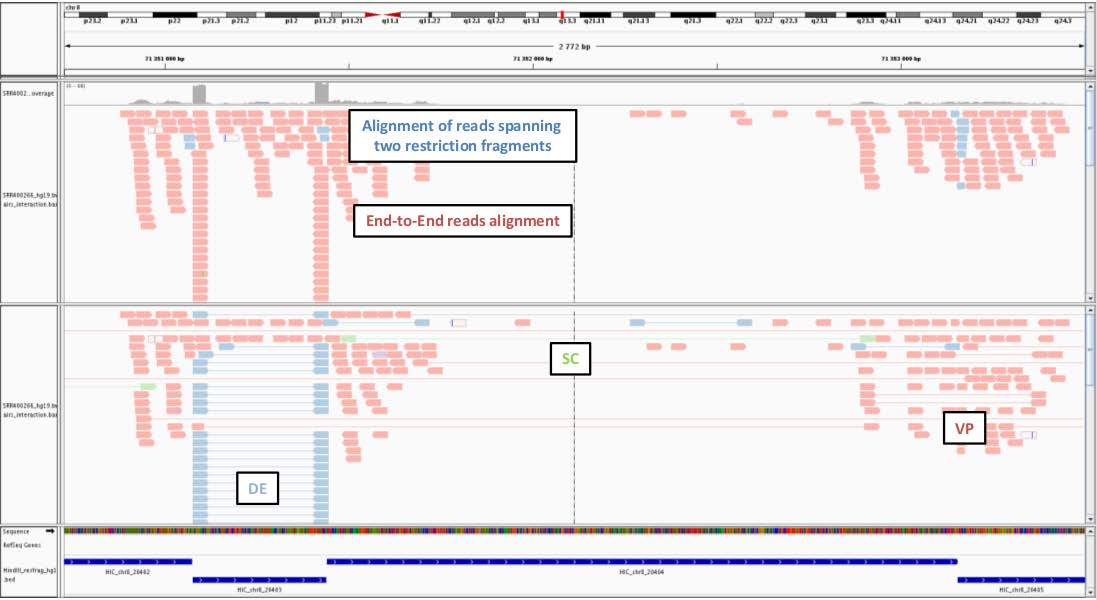
\includegraphics[width=\linewidth]{figures/suppfig1.png}
\caption{\bf IGV screenshot of BAM file after mapping and fragment
reconstruction.}{ Top panel. The reads are colored according to the alignment
procedure. Blue reads were trimmed before mapping, and flanked the restriction
fragment borders. Bottom panel. Read pairs are colored according to their
classification. Valid interactions are in red, dangling end in blue and
self-circle ligation in green.}
\label{suppfig:suppfig1}
\end{figure}

\begin{figure}
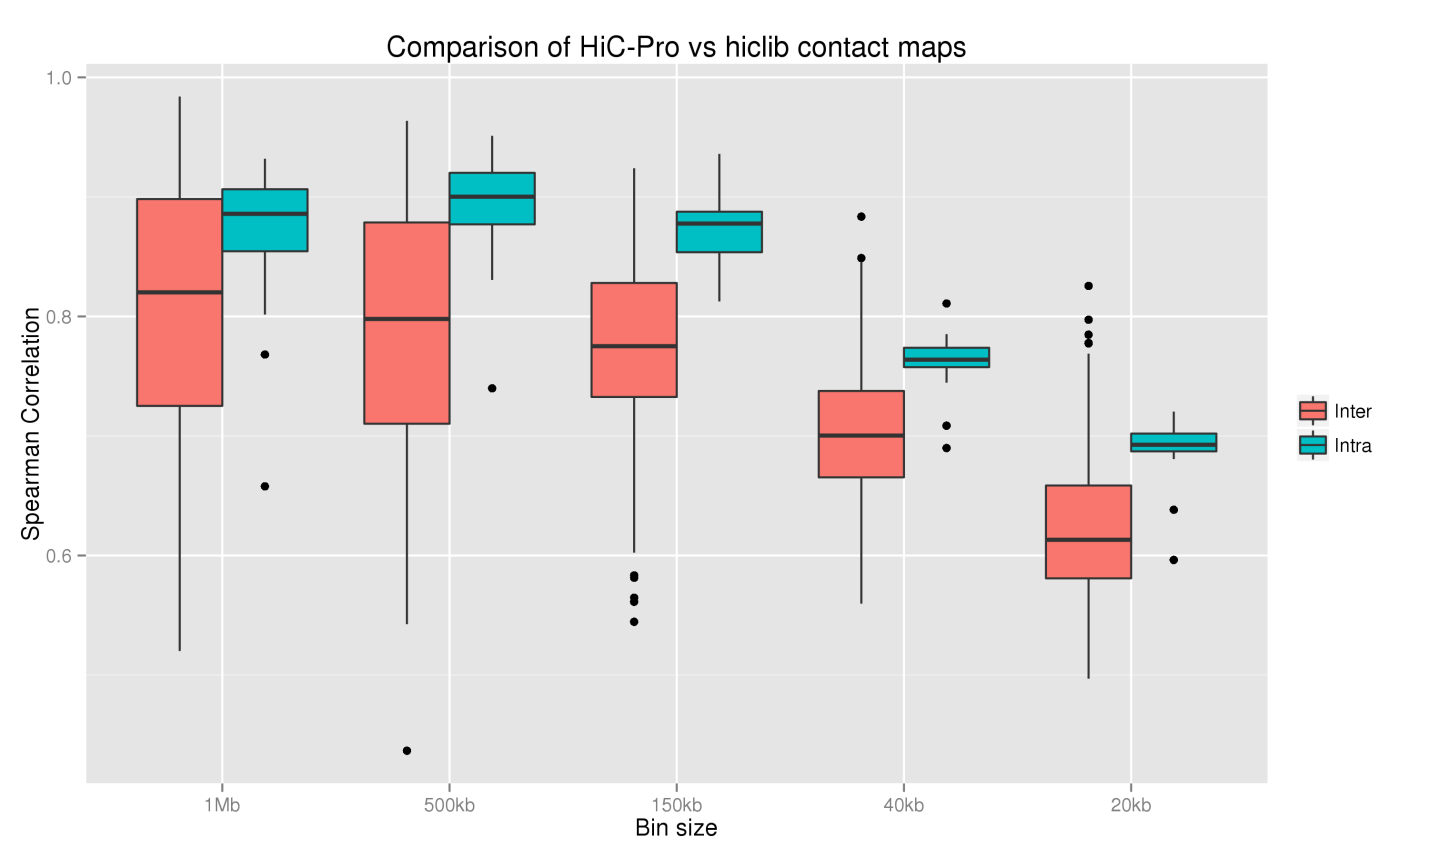
\includegraphics[width=\linewidth]{figures/suppfig2.png}
\caption{\bf Correlation of intra and inter-chromosomal contact maps generated
by hiclib and HiC-Pro.}{ Boxplots of the Spearman correlation coefficients of
intra and inter-chromosomal maps generated at different resolutions by both
pipelines.}
\label{suppfig:suppfig2}
\end{figure}
